%=============================================================================
% Thesis Template in LaTex
%
% File:  04-07-Kosten -- Analyse der Lösungen - Fallstudie
% Author(s): Jürgen Hackl <hackl@ibi.baug.ethz.ch>
%            Clemens Kielhauser <kielhauser@ibi.baug.ethz.ch>
%
% Creation:  27 Jan 2014
% Time-stamp: <Tue 2013-08-13 20:14 juergen>
%
% Copyright (c) 2014 Infrastructure Management Group (IMG)
%               http://ibi.ethz.ch
%
% More information on LaTeX: http://www.latex-project.org/
%=============================================================================

% Unterkapitel Kosten
% ---------

Die Abbildung \ref{img:Kostenberechnung} zeigt die Kostenberechnung der ersten 8 Jahre am Beispiel der Variante 1 im Szenario SB1/SU1. 
Die Ermittlung der Gesamtkosten einer Variante in einem Szenario erfolgt anhand der Berechnung der Zielfunktion, über den betrachteten Zeitraum von vierzig Jahren. Übersichtshalber zeige ich die Formel \ref{eq.x1} der Zielfunktion erneut.

\begin{equation}
Min. \thinspace K = Min. \thinspace [K_{W} + K_{B} + K_{TT} + K_{E} + K_{A}]
\label{eq.x1}
\end{equation} 

\begin{figure}[h!]
	\centering
	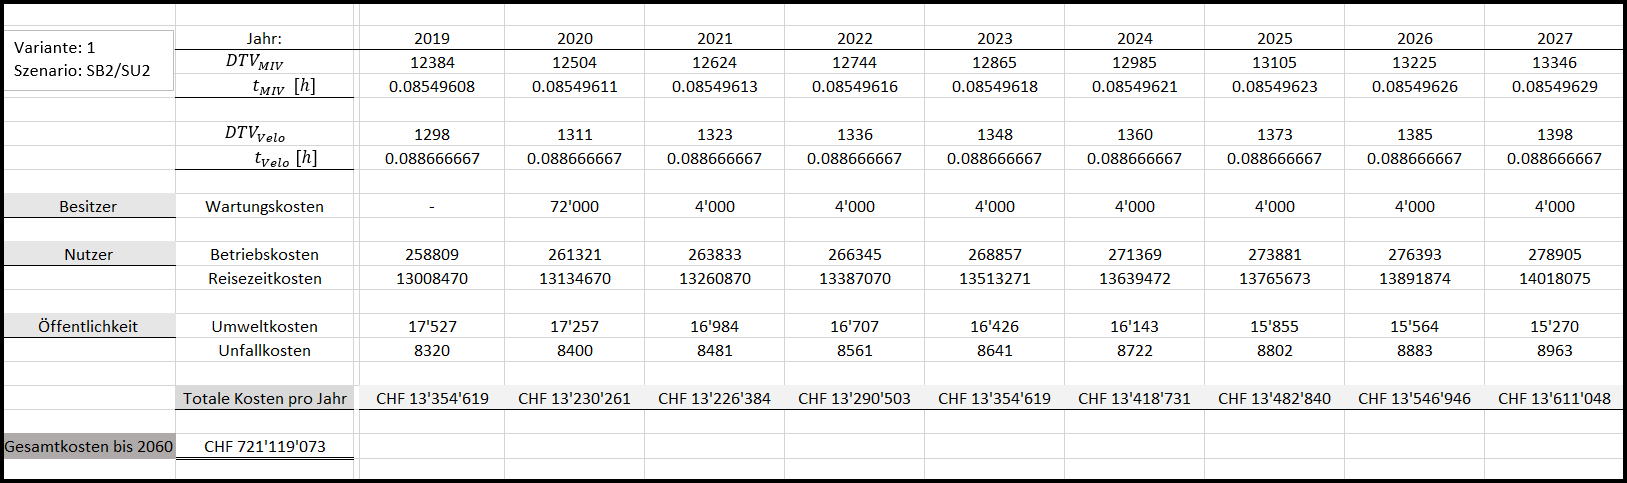
\includegraphics[width=\textwidth]{figures/f-04-06-04-Kostenberechnung}
	\caption[Kostenberechnung]{Beispiel der Kostenberechnung}
	\label{img:Kostenberechnung}
\end{figure}

Die jährlichen DTV Werte sind gemäss dem Abschnitt \ref{subsec:Modellierung} berechnet und die Reisezeitverluste $t$ gemäss Abschnitt \ref{sub:Reisezeit}. Nach \ref{sub:Unterhalt} werden die Wartungskosten berechnet. Die Berechnung der Wartungskosten erfolgt mit den in Abschnitt \ref{sec:Varianten} beschriebenen Abmessungen der Variante. Die im Jahr 2020 anfallenden Interventionskosten belaufen sich gemäss Abschnitt \ref{sec:Varianten} auf 68'000 CHF.

Die Betriebskosten der Nutzer werden gemäss Abschnitt \ref{sub:Betrieb} berechnet, dies erfolgt duch die Multiplikation des DTV mit der Länge der jeweiligen Fahrbahn und den Einheitskosten des Fahrzeugbetriebs. Um die Kosten eines Jahres zu ermitteln, wird der berechnet Wert mit 365 multipliziert. \\
Die weiteren Kosten der Nutzer sind die Reisezeitkosten, die nach Abschnitt \ref{sub:Reisezeit} berechnet werden. Hierfür wird der im oberen Bereich der Tabelle dargestellte Zeitverlust pro Nutzer, berechnet aus dem Zeitverlust, der durch das Befahren der Infrastruktur und durch die durchschnittliche Wartezeit aufgrund der Bahnschranke gemäss Abschnitt \ref{sub:Reisezeit} entsteht, mit dem DTV und den Einheitskosten des Zeitverlust, multipliziert.

Die Berechnung der Umweltkosten erfolgt nach Abschnitt \ref{subsec:Environment} durch die Multiplikation des DTV mit den Einheitskosten und der Länge der Fahrbahn. Im Fall der Schadstoffbelastungskosten wird, vom $DTV_{MIV}$ der jährliche E-Auto Anteil abgezogen.

Die Berechnung der Unfallkosten erfolgt pro Unfallkategorie und Fahrzeugtyp durch die Multiplikation des DTV mit der Länger der Fahrbahn den Unfallrisiken gemäss Abschnitt \ref{subsubsec:Unfallrisiko}. Daraus ergibt sich die jeweilige Unfallanzahl nach Unfallart. Diese werden mit den Einheitskosten der jeweiligen Unfallart multipliziert und die berechneten Kosten, um die totalen Unfallkosten zu ermitteln, aufsummiert. Im Anhang unter Abschnitt \ref{sec:Anhangkostenberechnug} sind die Tabellen der berechneten Kosten für die Varianten 1, 2 und 3 mit den Grundannahmen der Kostenstruktur aufgeführt.



% ===========================================================================
% EOF
%

%%% Local Variables:
%%% mode: latex
%%% TeX-master: "../main"
%%% End:
